\documentclass{ximera}
\usepackage{tkz-euclide}
\usetkzobj{all}
\begin{document}
\begin{problem}

  Suppose you cut a slice of pizza from a circular pizza of radius
  $r$, as shown.
  \begin{image}
      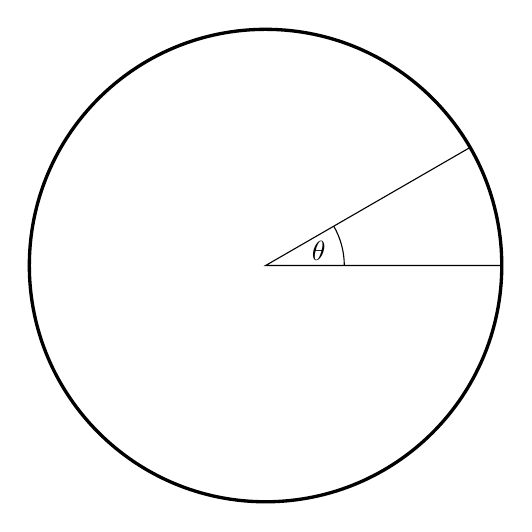
\begin{tikzpicture}
        \coordinate (O) at (0,0);
        \coordinate (A) at (3,0);
        \coordinate (B) at (3*.866,3*.5);
        \draw (A)--(O)--(B);
        \draw [very thick] (0,0) circle [radius=3];
        \tkzMarkAngle[size=1cm,thin](A,O,B)
        \tkzLabelAngle[pos = .7](A,O,B){$\theta$}
      \end{tikzpicture}
  \end{image}
  As you change the size of the angle $\theta$, you change the area of
  the slice, $A=\frac{1}{2}r^2\theta$. Then $A'$ is
  \begin{multipleChoice}
    \choice{constant.}
    \choice[correct]{$r\theta$}
    \choice{$\frac{1}{2}r^2$}
    \choice{not possible to determine from the given information.}
  \end{multipleChoice}
\end{problem}
\end{document}
